%%%%%%%%%%%%%%%%%%%%%%%%%%%%%%%%%%%%%%%%%%%%%%%%%%%%%%%%%%%
% EPFL report package, main thesis file
% Goal: provide formatting for theses and project reports
% Author: Mathias Payer <mathias.payer@epfl.ch>
%
% This work may be distributed and/or modified under the
% conditions of the LaTeX Project Public License, either version 1.3
% of this license or (at your option) any later version.
% The latest version of this license is in
%   http://www.latex-project.org/lppl.txt
%
%%%%%%%%%%%%%%%%%%%%%%%%%%%%%%%%%%%%%%%%%%%%%%%%%%%%%%%%%%%
\documentclass[a4paper,11pt,oneside]{report}
% Options: MScThesis, BScThesis, MScProject, BScProject
\usepackage[BScProject,lablogo]{EPFLreport}
\usepackage{xspace}
\usepackage{amsmath}

\title{Flatpak reproducibility (I will find a better title later)}
\author{Zacharie Timothée Tevaearai}
\supervisor{Flavio Toffalini}
\adviser{Prof. Dr. sc. ETH Mathias Payer}
%\coadviser{Second Adviser}
%\expert{The External Reviewer}

\newcommand{\sysname}{\emph{flatpak-rebuilder}\xspace}
\newcommand{\rb}{\emph{reproducible builds}\xspace}
\newcommand{\fp}{\emph{flatpak}\xspace}
\newcommand{\fh}{\emph{flathub}\xspace}
\newcommand{\fb}{\emph{flatpak-builer}\xspace}
\newcommand{\fdp}{\emph{flatpak dependencies}\xspace}
\newcommand{\sde}{SOURCE\_DATE\_EPOCH\xspace}
\newcommand{\fhbb}{\emph{flathub buildbot}\xspace}
\newcommand{\dfc}{\emph{diffoscope}\xspace}

\dedication{
    \begin{raggedleft}
        Ogey rrrrrrrat\\
        --- Pekora\\
    \end{raggedleft}
    \vspace{4cm}
    \begin{center}
        Dedicated.
    \end{center}
}

\begin{document}
\maketitle
\makededication

\begin{abstract}
Software can be built from source code or distributed as pre-compiled packages.
    These packages are the result of a software supply chain which can be
    subject to attacks or bugs and can not be trusted. A way to attest that a
    product from such a supply chain corresponds to its original source code is
    called \rb and consists in performing the exact build steps, for a certain
    package, independently of the main supply chain and compare the rebuilt
    artifact with the original one. If they are bit by bit identical, then we
    prove that the path between the source code and the final artifact is
    legitimate. Here we look at the possibility of using reproducible builds
    with \fp, a packaging technology used to ship the same binaries on multiple
    Linux distributions. In particular we focus on \fh, its main repository. We
    present a tool, called \sysname, which rebuild a package available on \fh,
    by recreating a minimal environment. We then measure the amount of
    reproducible packages, and further analyse their differences to understand
    the reasons of non-reproducibility and fix them.
\end{abstract}

\maketoc

%%%%%%%%%%%%%%%%%%%%%%
\chapter{Introduction}
%%%%%%%%%%%%%%%%%%%%%%

In theory, with free and open source software (FOSS) we can audit the code and
compile only software we trust. In reality most software is shipped as
pre-built binaries to end-users, through what is called a software
supply-chain. In this context how can we be sure that the result of such a
supply-chain is produced from the original source code ? Indeed, the
machine on which the software was compiled might be compromised, a bug may
occur during the process, or some maintainer may even be coerced into injecting
malicious code into the final product, there are all sort of reasons to not
trust what is shipped to the end-users. On top of that, auditing binaries is
much harder than auditing source code.
< Here I will quote a few papers and list a few example of software supply chain attack to give a bit more of context. >
One solution to attest that the path from source code to binary is correct, is
called \rb, which is a set of practises to make sure we can obtain the same
package, bit by bit, by reproducing the exact same build steps. If that is the
case, we can compare the results obtain by a set of independent rebuilder and
decide if we can trust the binaries or not \cite{DBLP:journals/corr/abs-2104-06020}.

One software distribution system that can benefit from \rb is \fp, and more
precisely its main repository called \fh. \fp is way to build, distribute and
deploy applications compatible on most Linux distributions. It works by running
applications inside of a container (which is referred as a sandbox) where they
have the minimum permissions and are as much isolated as possible from the host
system. Since the build is also performed inside the sandbox, it is an ideal
environment to use \rb, and \fp developers claim to have \rb, but this was not
yet proved.
< I can't find that claim anymore maybe I oversaw something >

In this project, we create a tool (\sysname) to allow individual to perform a
rebuild of a \fp from \fh, and attest if it produced the same artifact or not.
Using \sysname we then measure the reproducibility of \fp and provide
improvement to the \fh build infrastructure, in order to increase the amount of
reproducible programs. Since \fp works across Linux distribution, we also need
to develop a tool which is as portable, this limits the use of strong container
technologies, such as Docker, or tools such as \verb|faketime| to better
simulate the build environment.

<Continue by telling the main results and briefly explained the changes I
proposed to flatpak-builer and flatpak in general to have more reproducible builds>


%%%%%%%%%%%%%%%%%%%%
\chapter{Background}
%%%%%%%%%%%%%%%%%%%%

To better understand this project, we should introduce a bit more \rb,
especially the most common reasons a program may not be reproducible, but first
we define a build to be reproducible as such.
< Define what reproducible means for a program >
< Explain some reproducible builds concept >
< Explain flatpak >
< Explain flathub >

%%%%%%%%%%%%%%%%
\chapter{Design}
%%%%%%%%%%%%%%%%

\section{Recreating the environment}
To rebuild a program, \sysname must first make sure to gather all build
dependencies to the exact version used during the original build. There are two
types of dependencies defined in a \fb manifest file, the one which are
embedded in the final package, those are defined in the different
\emph{modules} of the manifest and their version is always perfectly defined.
For instance a dependency on a git repository will specify the hash of the
commit that need to be used. Those dependencies are therefore easy to gather
and is already done by \fb.
The other kind of dependency is what we refer to as \fdp, which include every
dependencies which are of the form of a flatpak, and will be mounted in the
sandbox during the build and sometimes also when running the final app. Those
dependencies include runtimes, sdk, sdk-extensions, base-app and base-app
extensions. In the case of \fh, these dependencies will come from \fh directly,
but the original manifest does not include the exact ostree commit associated
to each of these dependencies.
Fortunately, \fb will ship a modified version of the manifest in the final
product, which include the commit of the runtime, sdk, and (if there is any)
the base-app. Unfortunately it will not includes the one for sdk-extensions and
base-app extensions, but we know the \fhbb will use the latest one
available at the time of the build. However, the exact time of the build is
also not specified, it is bounded by the GitHub commit, which is before and the
ostree commit, which happens after the build.
We therefore guess which commit was used by taking the latest available at the
ostree commit time, this will introduce some error, but we will show that this
error is relatively small.
Another dependency we need to pin to its exact version is \fb itself, in the
case of the \fhbb, it uses the one available on \fh, we therefore
consider it as any other \fdp, and apply the same guessing technique.

Under the hood, \fb override the \sde environment variable with the last
modification time of the manifest file, but this information is lost when a
file is committed to git or ostree, we therefore do as before, and use the
ostree commit time to override the \sde, which is another source of error, but
we cannot do better for now.

\section{Rebuilding}
Once the environment matches roughly the one from the original build, we need
to execute the exact same steps done by the \fhbb. Since its code is
open-source, we merely follow the same code, we just ignore the verification
and exporting steps done at the end.

\section{Measuring reproducibility}
At the end of a rebuild we compare the hash of the original package, with the
rebuilt one and conclude that the build is reproducible if the two are the
same. This follows a very strict definition of reproducibility and we therefore
introduce three more notions, two binary and a continuous one (that's not the
term but whatever). The first is the notion of binary-reproducibility, where we
compute the hash of only non human-readable files (ELF, images, archives, etc.)
the second is ELF-reproducibility, where we only compare ELF files, and the
last one is the repro-score, which is defined as the number of non-reproducible
files over the total number of files.
The reasoning behind the binary and ELF reproducibility is the following: we
can still audit and understand non binary files, and therefore if the only
sources of non-reproducibility are in files we can easily verify manually, we
can still attest that the build is legitimate, even it is only partially
reproducible.
The idea behind the repro-score is to find a way to characterize a program
which is highly non-reproducible, from those which are mostly reproducible, by
assuming that a program with a high repro-score will be easy to fix, and make
reproducible.


%%%%%%%%%%%%%%%%%%%%%%%%
\chapter{Implementation}
%%%%%%%%%%%%%%%%%%%%%%%%

The implementation covers some of the implementation details of your project.
This is not intended to be a low level description of every line of code that
you wrote but covers the implementation aspects of the projects.

This section is usually 3-5 pages.

< I will do this part later I think, I am not yet sure what I should put >

%%%%%%%%%%%%%%%%%%%%
\chapter{Evaluation}
%%%%%%%%%%%%%%%%%%%%

\section{Current reproducibility of \fh}
We evaluate the reproducibility of \fh by running our code on as many
applications as possible. As of \today, \fh contains 1728 programs, classified
as an application (by opposition with runtimes). We only focus on applications
because those are built using the \fhbb. In order to save time, we only rebuild
729 of them and got the following results:

\begin{table}[h]
    \centering
        \begin{tabular}{|c|c|c|c|}
            \hline
            & Reproducible & Non reproducible & Failed\\
            \hline
            All & 306 & 368 & 55\\
            \hline
            All\% & 42\% & 50.5\% & 7.5\% \\
            \hline
            ELF & 423 & 251 & 55\\
            \hline
            ELF\% & 58\% & 34.5\% & 7.5\% \\
            \hline
        \end{tabular}
    \caption{Reproducibility over 729 programs}
    \label{tab:rebuild-all}
\end{table}

< I should specify here that ELF reproducibility was not exactly matching the definition I gave before (because the code was a bit naive at that moment) >

As a comparison, at the same time, Arch Linux has 86.4\% reproducibility on
their repository\cite{arch-rebuilderd}. We observe poor reproducibility
performances in comparison. Two source of error are already known, first, some
dependencies versions are guessed and second the exact time of the build is
uncontrolled. We can approximate the probability of the first error in the
following way: The time of the GitHub commit and ostree commit are known, and
the build must happen in between. We make a commit guessing error when an
update of one dependency we need to guess is published between the start of the
build and the ostree commit. If we assume that the start of the build is
uniformly distributed between the GitHub commit $GH_{commit}$ and the ostree
commit $OT_{commit}$, then we make an error when the start is behind the update
of the dependency closest to $OT_{commit}$:
\begin{align}
    P_{error} &= \max_{d \in Dependencies}(P_{error\_guessing\_d}) \\
              &= \max_{d}
              \begin{cases}
                \frac{OT_{commit} - d_{update}}{OT_{commit} -
                    GH_{commit}}  & \quad \text{if } d_{update}
                    \in [GH_{commit}; OT_{commit}] \\
                0  & \quad \text{if } d_{update}
                  \notin [GH_{commit}; OT_{commit}]
              \end{cases}
\end{align}
The expected value of this upper-bound on all apps on \fh is $19.6$, our
guessing techniques is therefore accurate and cannot explain the amount of
non-reproducible programs.


\section{Theoretical reproducibility}
\label{sec:theo-repro}
To better understand \autoref{tab:rebuild-all}, we design this experiment, we
rebuild a fraction of the non reproducible programs, twice, on two different
setups, and see if we obtain the same checksum on both. If that is the case,
the program can be considered as theoretically reproducible, because this means
it should be reproducible but the way it is rebuilt by \sysname is not matching
enough what is done by the \fhbb. Instead of rebuilding everything we again
reduce the number of program we consider, to save time. The time to rebuild a
program can be characterize as such: $\frac{deps}{internet speed} + rebuild
time$, and we can reduce the total amount of building time by 2 by removing 7\%
of them as shown in \autoref{fig:buildtime}.

\begin{figure}[h]
    \center{
        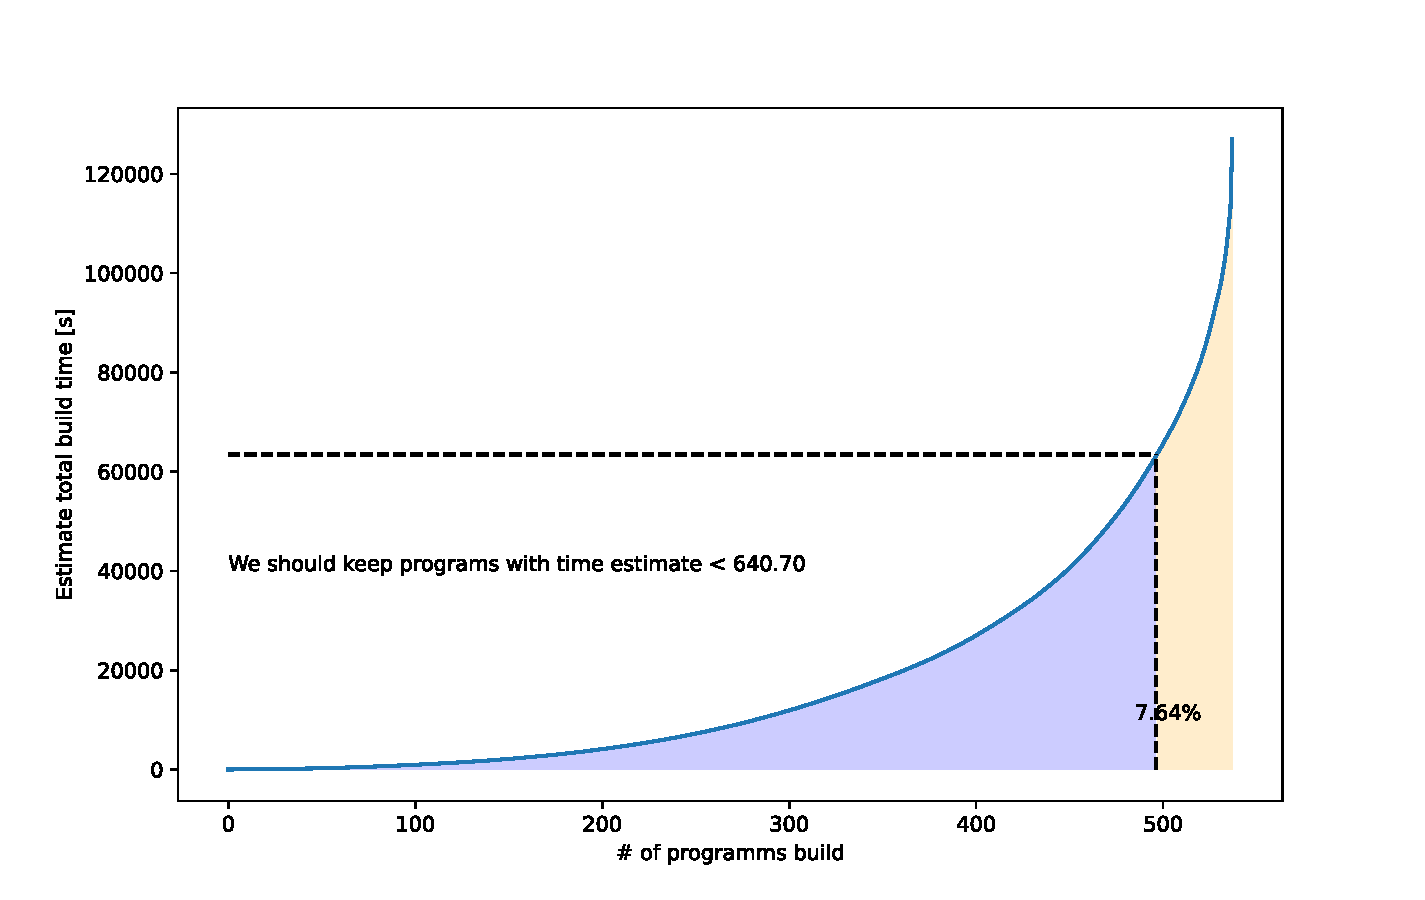
\includegraphics[width=\textwidth]{figures/buildtime.pdf}
    }
    \caption{Cumulative build time, 7.64\% of programs
    account for half of the total build time, we therefore remove them.}
    \label{fig:buildtime}
\end{figure}

By building twice 185 programs, 70 of them (37.6\%) are in theory reproducible,
and 73 are binary-reproducibility. The code that evaluate ELF-reproducibility
was buggy at that moment (and I'm still angry about it). <I won't put that in
the final product>
If we extrapolate from that sample we conclude that we could reach 61\%
reproducibility by better mimicking the original build environment.

\section{Kind of non reproducibility}
To better explain why these program are not reproducible, and also why some of
them should be in theory, we manually analyse each result and label the most
common pattern we see. To save time again, we only consider the 185 ones that
were rebuilt in section \autoref{sec:theo-repro}. To perform the analysis look
at the difference between the two artifacts using \dfc, a tool that perform
deep diffing analysis, created in the context of the \rb project.

\subsection{Timestamps}
18 of the 185 programs have timestamps embedded in their static strings, or in
some files metadata, like images or archives, but they are equal to the value
of \sde, meaning that it is easy to manipulate them. Furthermore 24 programs
have what we call absolute timestamps embedded in the final package. Absolute
timestamps are not controlled by \sde, and we therefore \sysname cannot force
their value.

\subsection{Debug link}
When applicable, debug symbols of a program on \fh are available, as an
extension. In order to do so, debug symbols are stripped and put in a separate
\emph{gnu\_debuglink} file, and a section called .gnu-debug-link is added to the
source ELF binary. This section contains the path to the debug symbol file, and
a checksum of this file, this checksum is a typical source of
non-reproducibility, 63 of the analysed programs are affected.


\subsection{Resolved manifest serialisation}
< TODO >

\subsection{.ro\_data}
The .ro\_data section is a common location of non-reproducibility, first
because it includes static strings that may have timestamps or path information
in them, but there is another common pattern shown in \autoref{fig:rodata}.
Some section only differ at some bytes, with always the same difference.
< That's a bad explanation I should redo it >
< It could be some padding or some uninitialized value maybe ??? Still need to investigate. >
\begin{figure}[h]
    \center{
        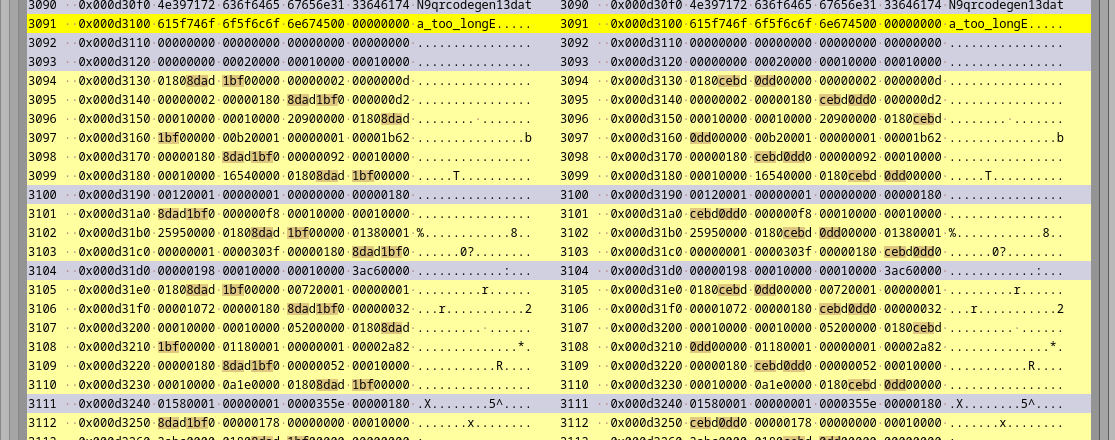
\includegraphics[width=\textwidth]{figures/random_ro_diffoscope.png}
    }
    \caption{Example of \dfc output on a program which differ in the .ro\_data section, with the same pattern, the same 28bits separate by 148bits each time}
    \label{fig:rodata}
\end{figure}

\subsection{Python files}
< TODO >

\subsection{Path}
< TODO >

\subsection{Hardware dependant compilation}
< TODO >

\subsection{Appstream}
< TODO >

\section{Time influence}
To better understand how time influence a build, we add an option to manipulate
the time of the build used by \sysname and we observe the following things.
Obviously timestamps which match the \sde variable change but so do the
\emph{.ro\_data} sections and the \emph{.gnu\_debuglink}.
< If I have time I should figure out why it is the case >

\section{Repro score analysis}
< I'm rerunning the experiment >


%%%%%%%%%%%%%%%%%%%%%%%%%%%%
\chapter{Improvement design}
%%%%%%%%%%%%%%%%%%%%%%%%%%%%
< New section, will describe how I use previous result to improve \sysname and \fb >

%%%%%%%%%%%%%%%%%%%%%%%%%%%%%%%%
\chapter{Improvement evaluation}
%%%%%%%%%%%%%%%%%%%%%%%%%%%%%%%%
< New section, if I have time, will evaluate the improvement from previous section >


%%%%%%%%%%%%%%%%%%%%%%
\chapter{Related Work}
%%%%%%%%%%%%%%%%%%%%%%

The related work section covers closely related work. Here you can highlight
the related work, how it solved the problem, and why it solved a different
problem. Do not play down the importance of related work, all of these
systems have been published and evaluated! Say what is different and how
you overcome some of the weaknesses of related work by discussing the
trade-offs. Stay positive!

This section is usually 3-5 pages.


%%%%%%%%%%%%%%%%%%%%
\chapter{Conclusion}
%%%%%%%%%%%%%%%%%%%%

In the conclusion you repeat the main result and finalize the discussion of
your project. Mention the core results and why as well as how your system
advances the status quo.

\cleardoublepage
\phantomsection
\addcontentsline{toc}{chapter}{Bibliography}
\printbibliography

\end{document}
